\documentclass[a4paper]{article}
\usepackage{xeCJK, indentfirst}
\usepackage{amsthm,amssymb,amsmath}
\usepackage{graphicx, subfigure}
\setCJKmainfont{AR PL UMing TW MBE}
\title{火の人工知能玄 Report}
\author{Group 8 鄭余玄、謝昀佐、陳令原}
\date{}
\begin{document}
\maketitle
\section{前言}
這次的 final project 規定是建立一個 Bayesian Belief Network 並且使用 MCMC 方法去解決一個問題。因此我們這組決定跨領域整合,試圖 model 一個真實世界的問題,而不只是能交作業用的 toy problem。2016 年嚴重受到聖嬰現象影響,在新聞報導中時不時會出現森林大火相關報導。此外,森林大火同時也是森林管理一項十分重要的課題,所以我們這組決定以此作為研究主題。

森林大火是一個牽涉很廣泛的問題,如圖~\ref{ffp}主要成三部分,分別是森林大火的發生、危害以及後果。研究森林大火的發生成因,需要透過實地田野調查、氣象觀測站、火災數據或相關預報指數等等,收集這些時空資料到 GIS 資料庫中。接著,利用資料所形成的時間和空間機率分布,去訓練出模型進行預測。而此預測的最終目的是,能夠評估火災所帶來的危害,這也是森林大火事件最關心的問題,因為這已經不只影響當地的居民,更擴及到投資人的經濟損失。

\begin{figure}[h]
  \caption{Forest Fire Analysis}
  \centering
  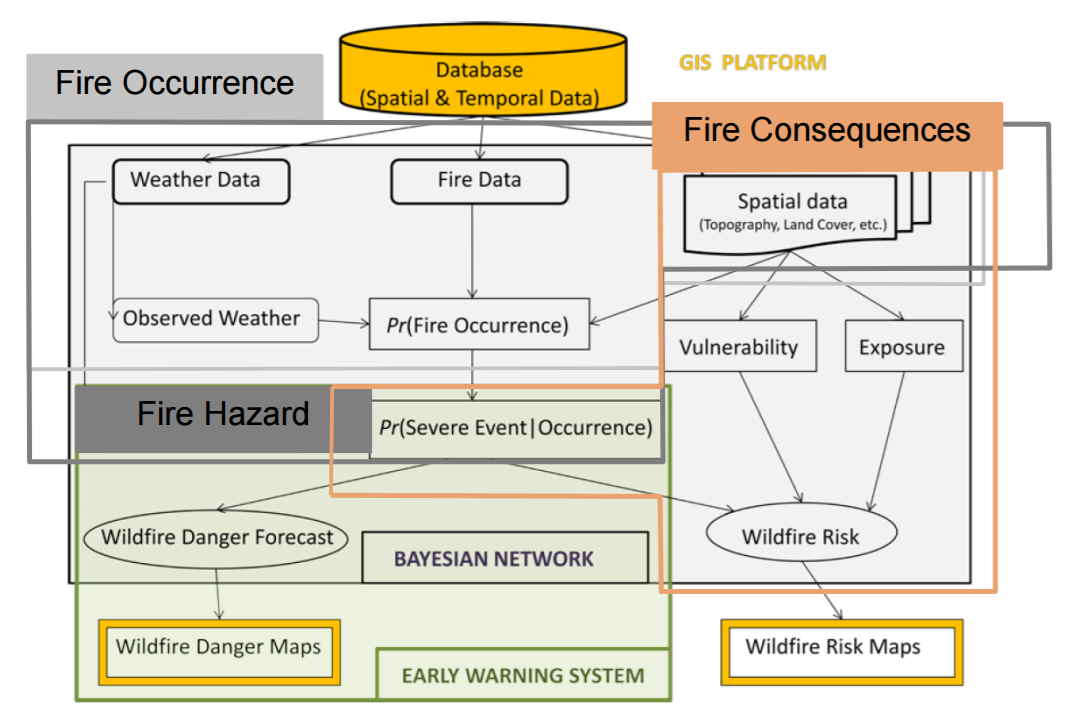
\includegraphics[width=1\textwidth]{problem}
  \label{ffp}
\end{figure}

\section{理論運用}
森林大火的成因分析主要是依據韓國慶州市的一篇研究~\cite{MCFFSK},實地利用異質空間點過程 SPP 去建立森林起火密度模型。再搭配地景、地形起伏、山坡斜率、植被,去進行區域互動共變異影響,建立一個比使用帕松點過程還好的空間邏輯迴歸模型。

繼參考數篇森林大火成因之後,另一篇德國的論文~\cite{BBN}則是討論如何利用這些成因去建立可以自動 structure learning 的 BBN~\cite{Model},最後再使用 NBC 去作驗證。這篇論文最終的模型是如圖~\ref{bbn_proto},其中目標節點是燃燒面積,而虛線的隨機變數是屬於 hidden variable。

\begin{figure}[h]
  \caption{A BBN model for predicting wildfire spreading}
  \centering
  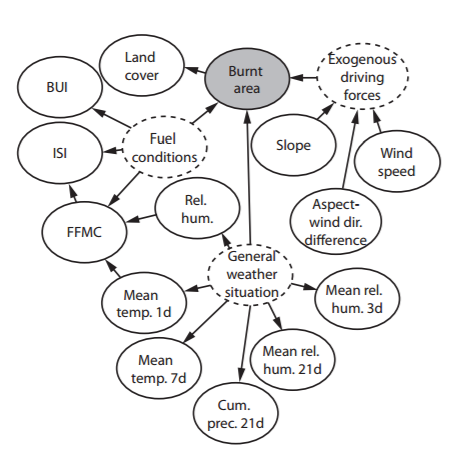
\includegraphics[width=.78\textwidth]{bbn_proto}
  \label{bbn_proto}
\end{figure}

基於實作的可能性,我們將資料簡化,因此資訊的萃取僅採取以FFMC(細小易燃物濕度指數)、DMC(腐植質濕度指數)、DC(乾旱指數)、ISI(初始蔓延速率)、temp(溫度)、RH(相對溼度)、wind(風速)、rain(降雨量)、area(面積)做為一般的隨機變數(random variable),而分別透過DMC、DC生成BUI(累積指數),再由BUI、ISI與FFMC生成Fuel(可燃物指數),以及RH、rain生成Weather(天氣指數)這三個hidden variables,其 BBN 如圖~\ref{bbn} 所示。

其中,FFMC(Fine Fuel Moisture Code,細小易燃物濕度指數)係指易燃物(Fine Fuel)中,含水成分的比例。此指數可以顯示易燃物的可起火性與可燃性。DMC(Duff Moisture Code,腐植質濕度指數)則係指在地層的O層(Organic Layer,有機層)中度深度中的平均濕度。此指數可以顯示中度深度中,可燃燒的中等大小木頭。DC(Dought Code,乾旱指數)是在O層深層中的平均濕度。此指數可以顯示可悶燒的物質。而ISI(Initial Spread Index,初始蔓延速率)則是火蔓延的期望速率,可以顯示不考慮可燃物量的時候,火勢蔓延的情形。另外,BUI(Buildup Index,累積指數)是指可燃物的累積的總量比例。

\begin{figure}[h]
  \caption{BBN}
  \centering
  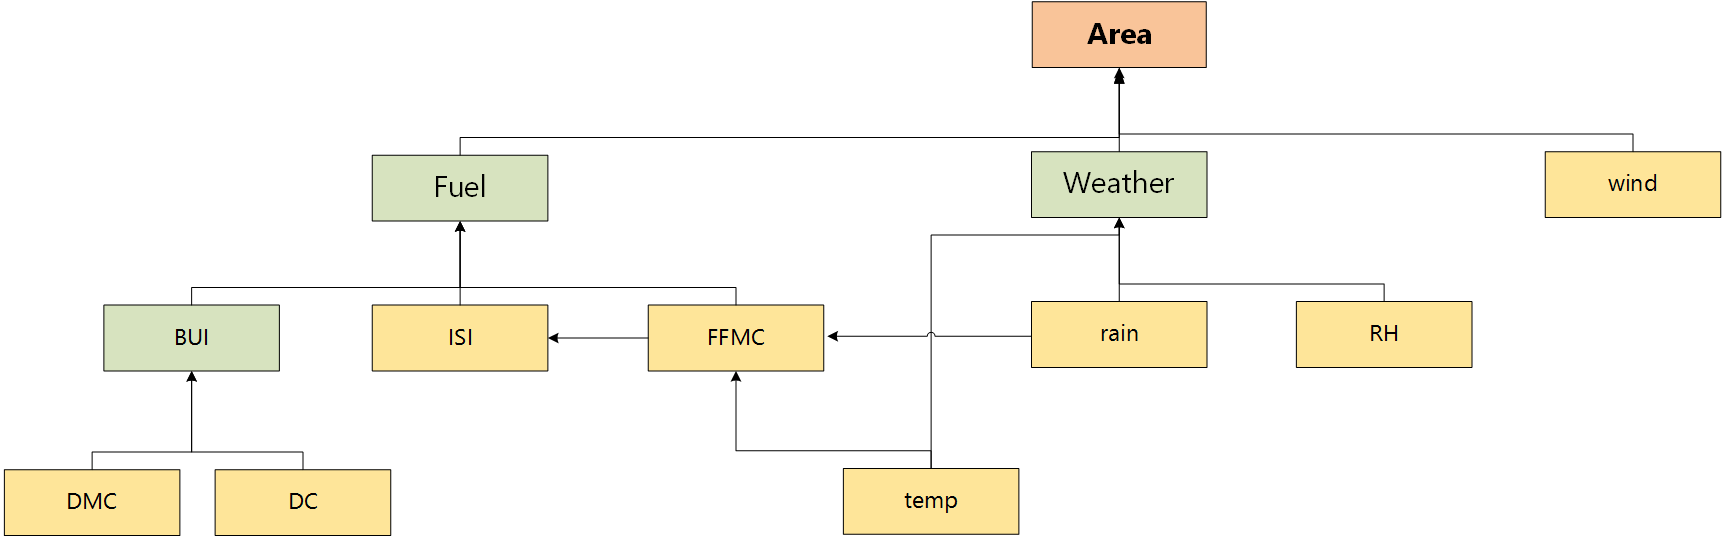
\includegraphics[width=1\textwidth]{bbn}
  \label{bbn}
\end{figure}

\section{實作過程}
因為森林大火我們這組沒有辦法自行蒐集到有效而且完整的資料,所以我們花了需多時間在研究如何形成一個合理並且符合現實情況的模型。我們實作是使用 UCI 機器學習倉儲的森林大火資料集~\cite{UCIFF},接下來的實作步驟是 model 每個節點,連接這些節點形成 BBN,並且計算出 Conditional Probability Table (CPT),最後使用 MCMC 在機率網路上作 inference。此外,為了驗證程式的正確性,我們有實作常見的 rain model,來確保程式碼是正確執行的,並且以 7:3 比例分配原始資料集作訓練和驗證。

因為這個資料集的燃燒面積偏小,我們推測是因為該地區的植被和降雨量的影響,但是這可能會造成計算時的浮點位數誤差,因此參考使用這個資料集的論文~\cite{dataset},我們一樣使用$\log(X+1)$變換,擴大數值之間的差距如圖~\ref{area}。

\begin{figure}[h]
  \caption{Area transformation}
  \centering
  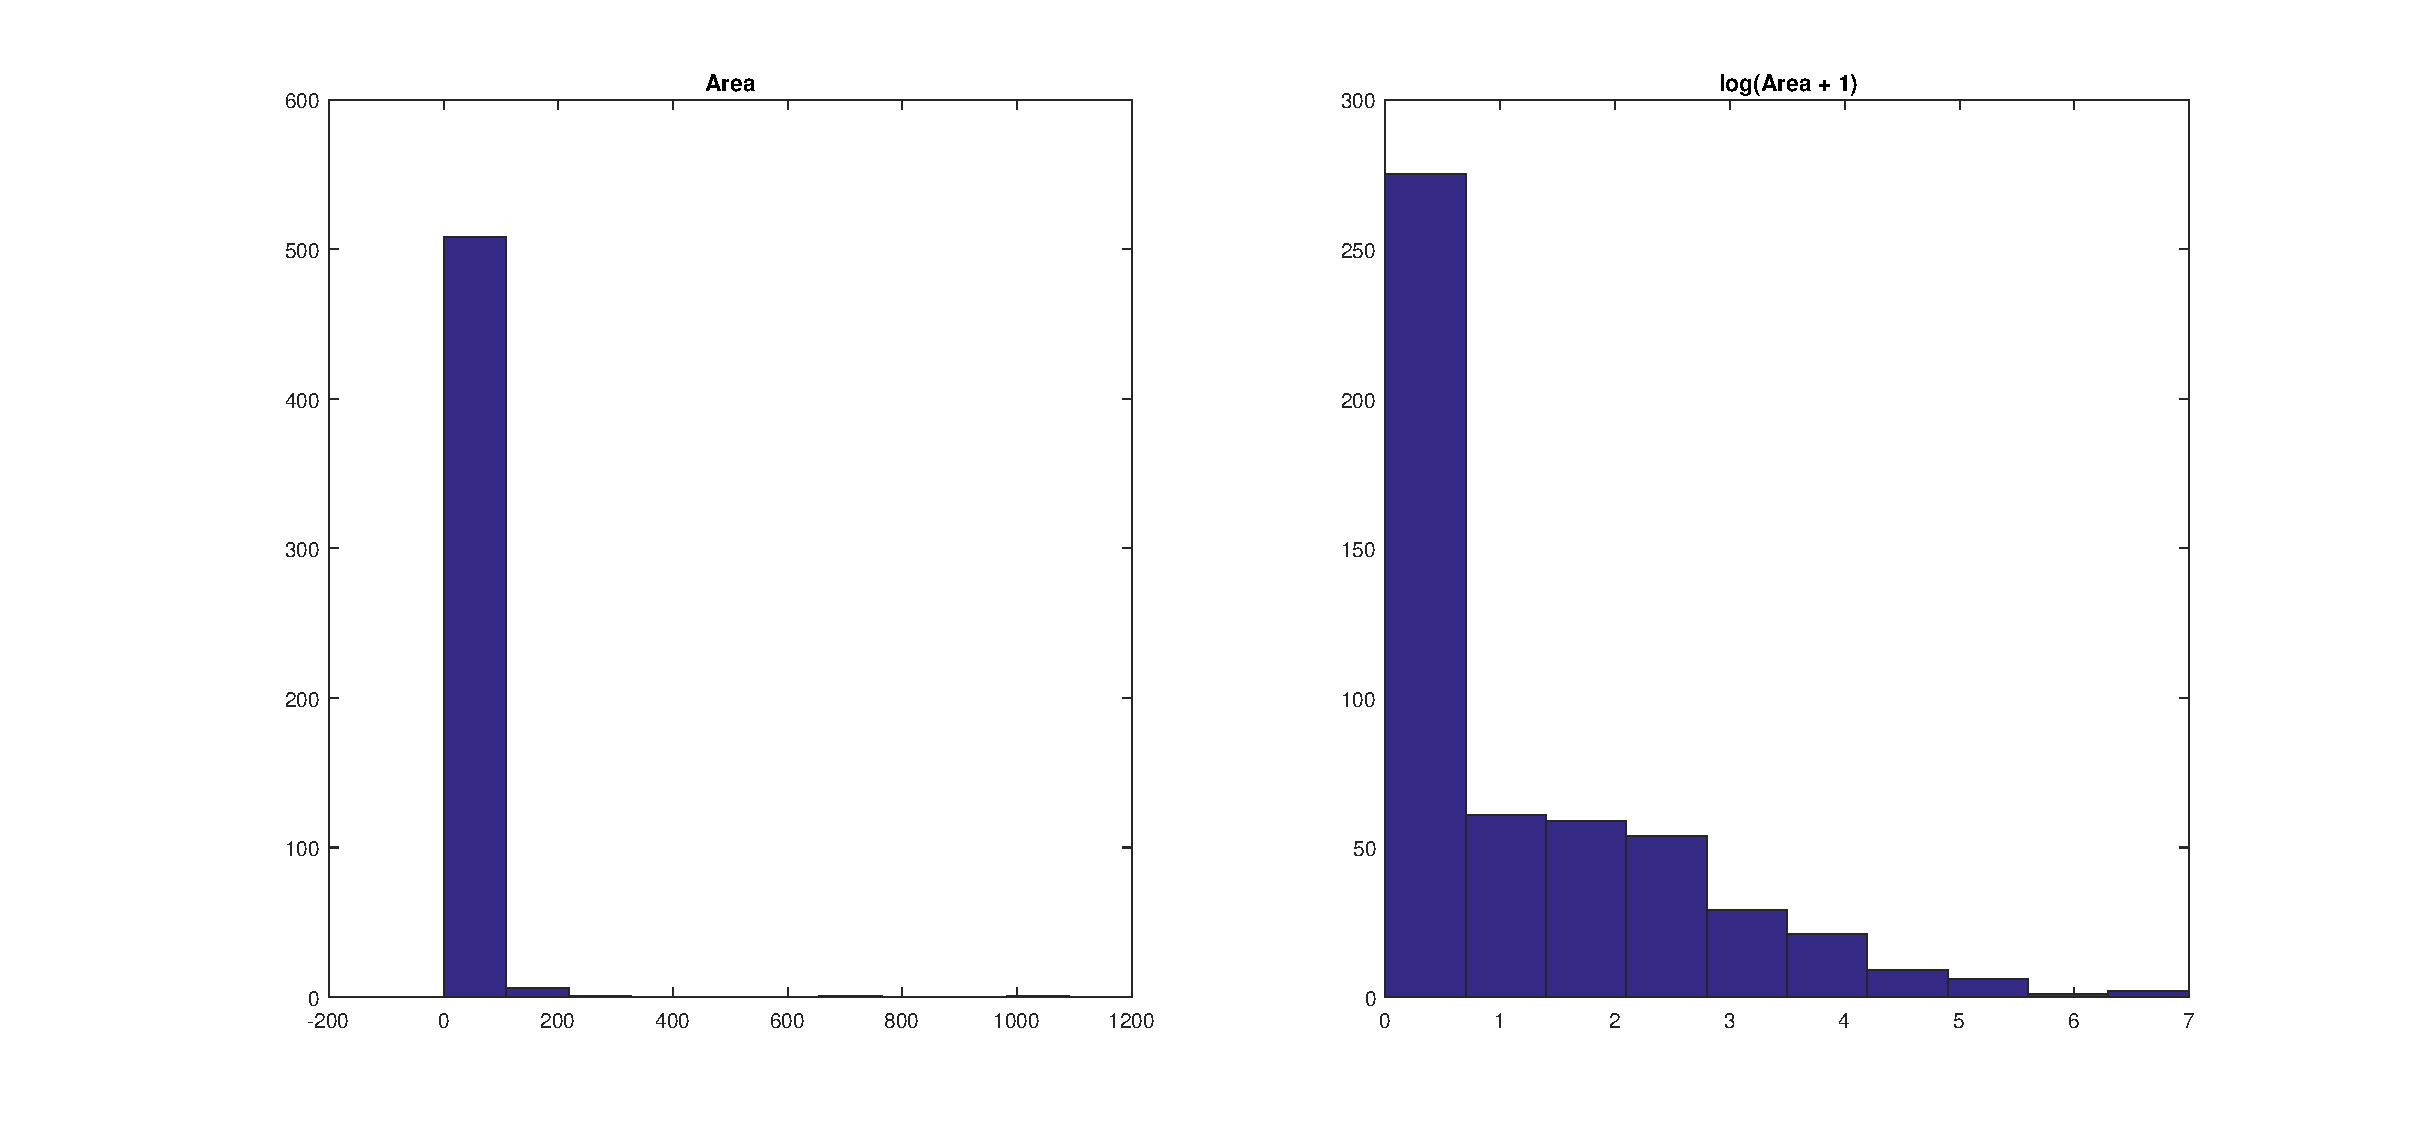
\includegraphics[width=1\textwidth]{area}
  \label{area}
\end{figure}

當我們這組分析完整個專案之後,因為考慮到需要使用大量數值計算,所以我們這組決定使用 MATLAB 來實作。程式碼的實作大部分是參考 The Bayes Net Toolbox for Matlab~\cite{bnet}。考慮到整個機率網路是十分複雜的,因此會假設隨機變數之間是馬可夫鏈,並且使用 Gibbs sampler 去實作 Markov Chain Monte Carlo 估計機率推論。

\section{實驗}
一開始我們這組實作的機率網路比 report 上的還要複雜許多,包括每個節點都預設是連續機率變數,之間的條件機率也是連續的分布。但是每次要進行實驗的時候,電腦跑一跑就會因為記憶體被佔滿就當機了\footnote{Memory: 12.0 GB DDR3; CPU: Intel (R) Core(TM) i7-4720HQ CPU @ 2.60GHz}。後來只好到使用實驗室的電腦去 train BBN 的參數,雖然記憶體足夠使用了\footnote{Memory: 15.0 GB DDR3}如圖~\ref{ram},但是電腦無法負荷計算太大量的節點資訊如圖~\ref{param}。因此這是實驗主要受到許多計算資源的限制,不論是在實作上盡量以空間換取時間,但是又過猶不及,最後才改進到報告中的模型。

最後實驗結果如圖~\ref{result},我們驗證了 155 筆不同的情形對比資料庫的 ground truth,程式判斷正確率接近七成,再加上計算時間已經調校到約兩秒鐘左右,我們這組認為結果已經想當不錯了。

\begin{figure}[h]
  \caption{Result}
  \centering
  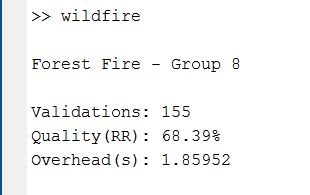
\includegraphics[width=.7\textwidth]{result}
  \label{result}
\end{figure}

\begin{figure}[h]
  \caption{RAM limitation}
  \centering
  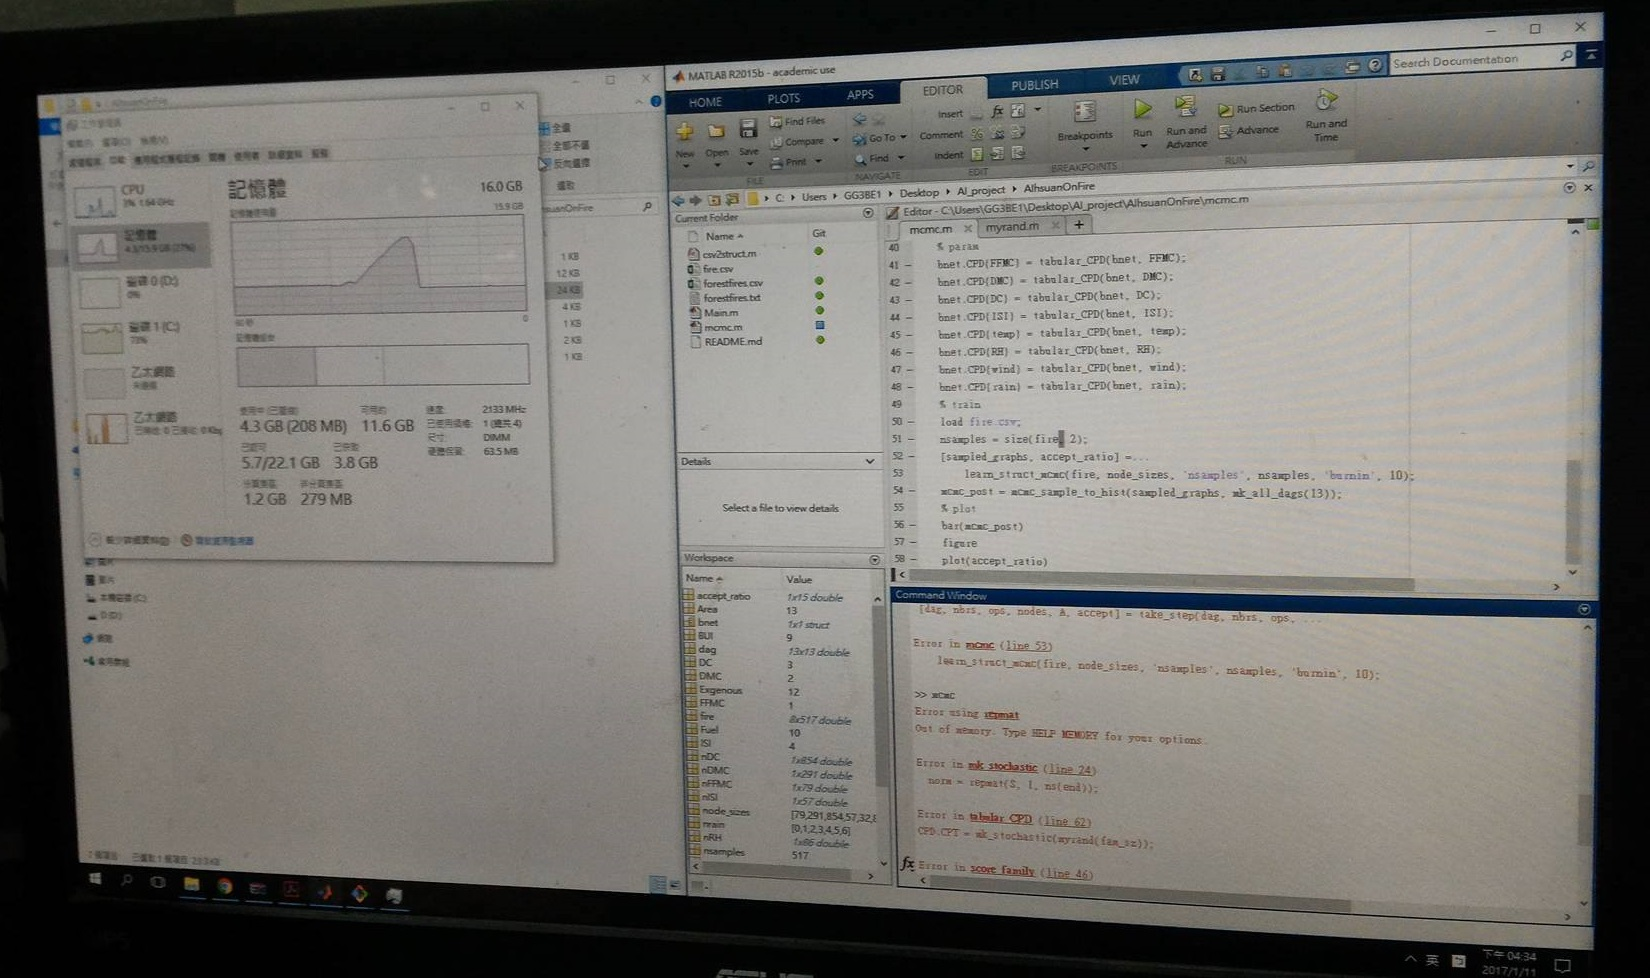
\includegraphics[width=1\textwidth]{RAM}
  \label{ram}
\end{figure}

\begin{figure}[h]
  \caption{Node Parameters}
  \centering
  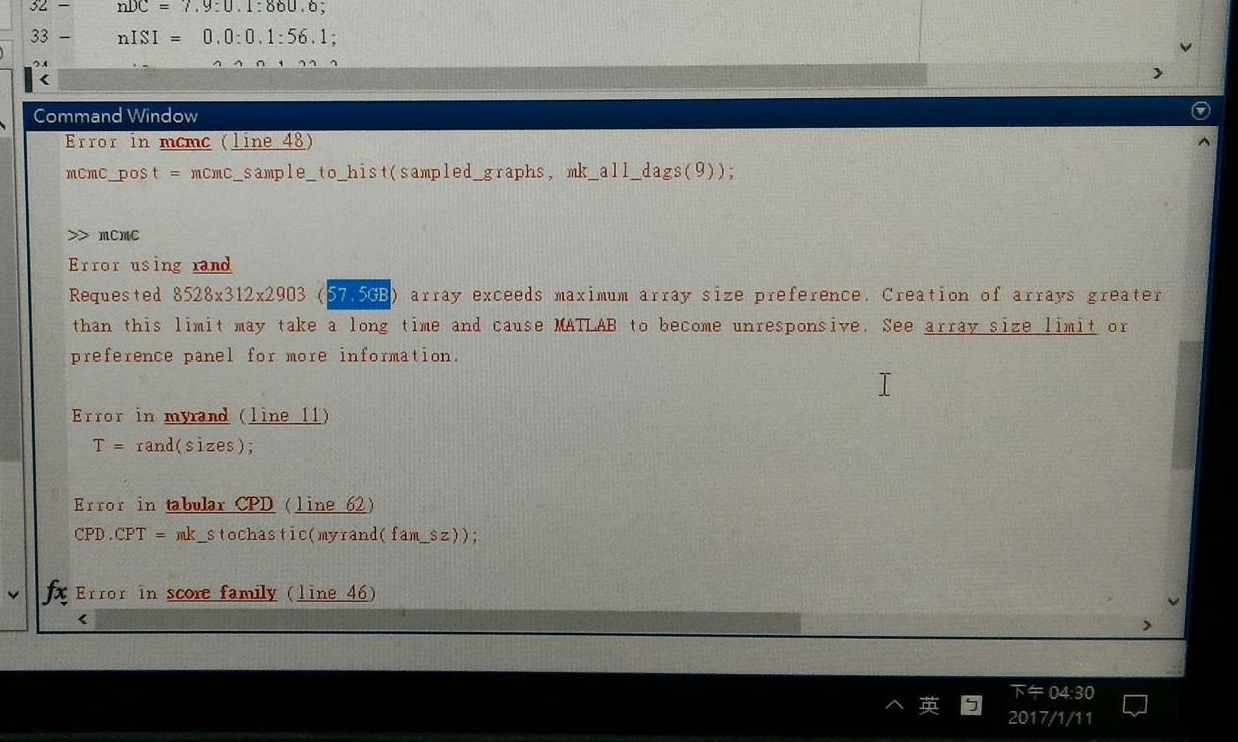
\includegraphics[width=1\textwidth]{57GB}
  \label{param}
\end{figure}

\bibliographystyle{IEEEtran}
\bibliography{./refs}
\end{document}